\documentclass{article}
\usepackage[utf8]{inputenc}
\usepackage[T1]{fontenc}
\usepackage{tikz}
\usetikzlibrary{arrows.meta,positioning,fit,shapes.multipart,shapes.geometric,shadows}
\usepackage{amsfonts}
\usepackage{amsmath}
\usepackage{amssymb}
\usepackage{graphicx}
\usepackage{float}
\usepackage[dvipsnames]{xcolor}

\begin{document}

\begin{figure}[H]
  \centering
  \resizebox{\textwidth}{!}{%
  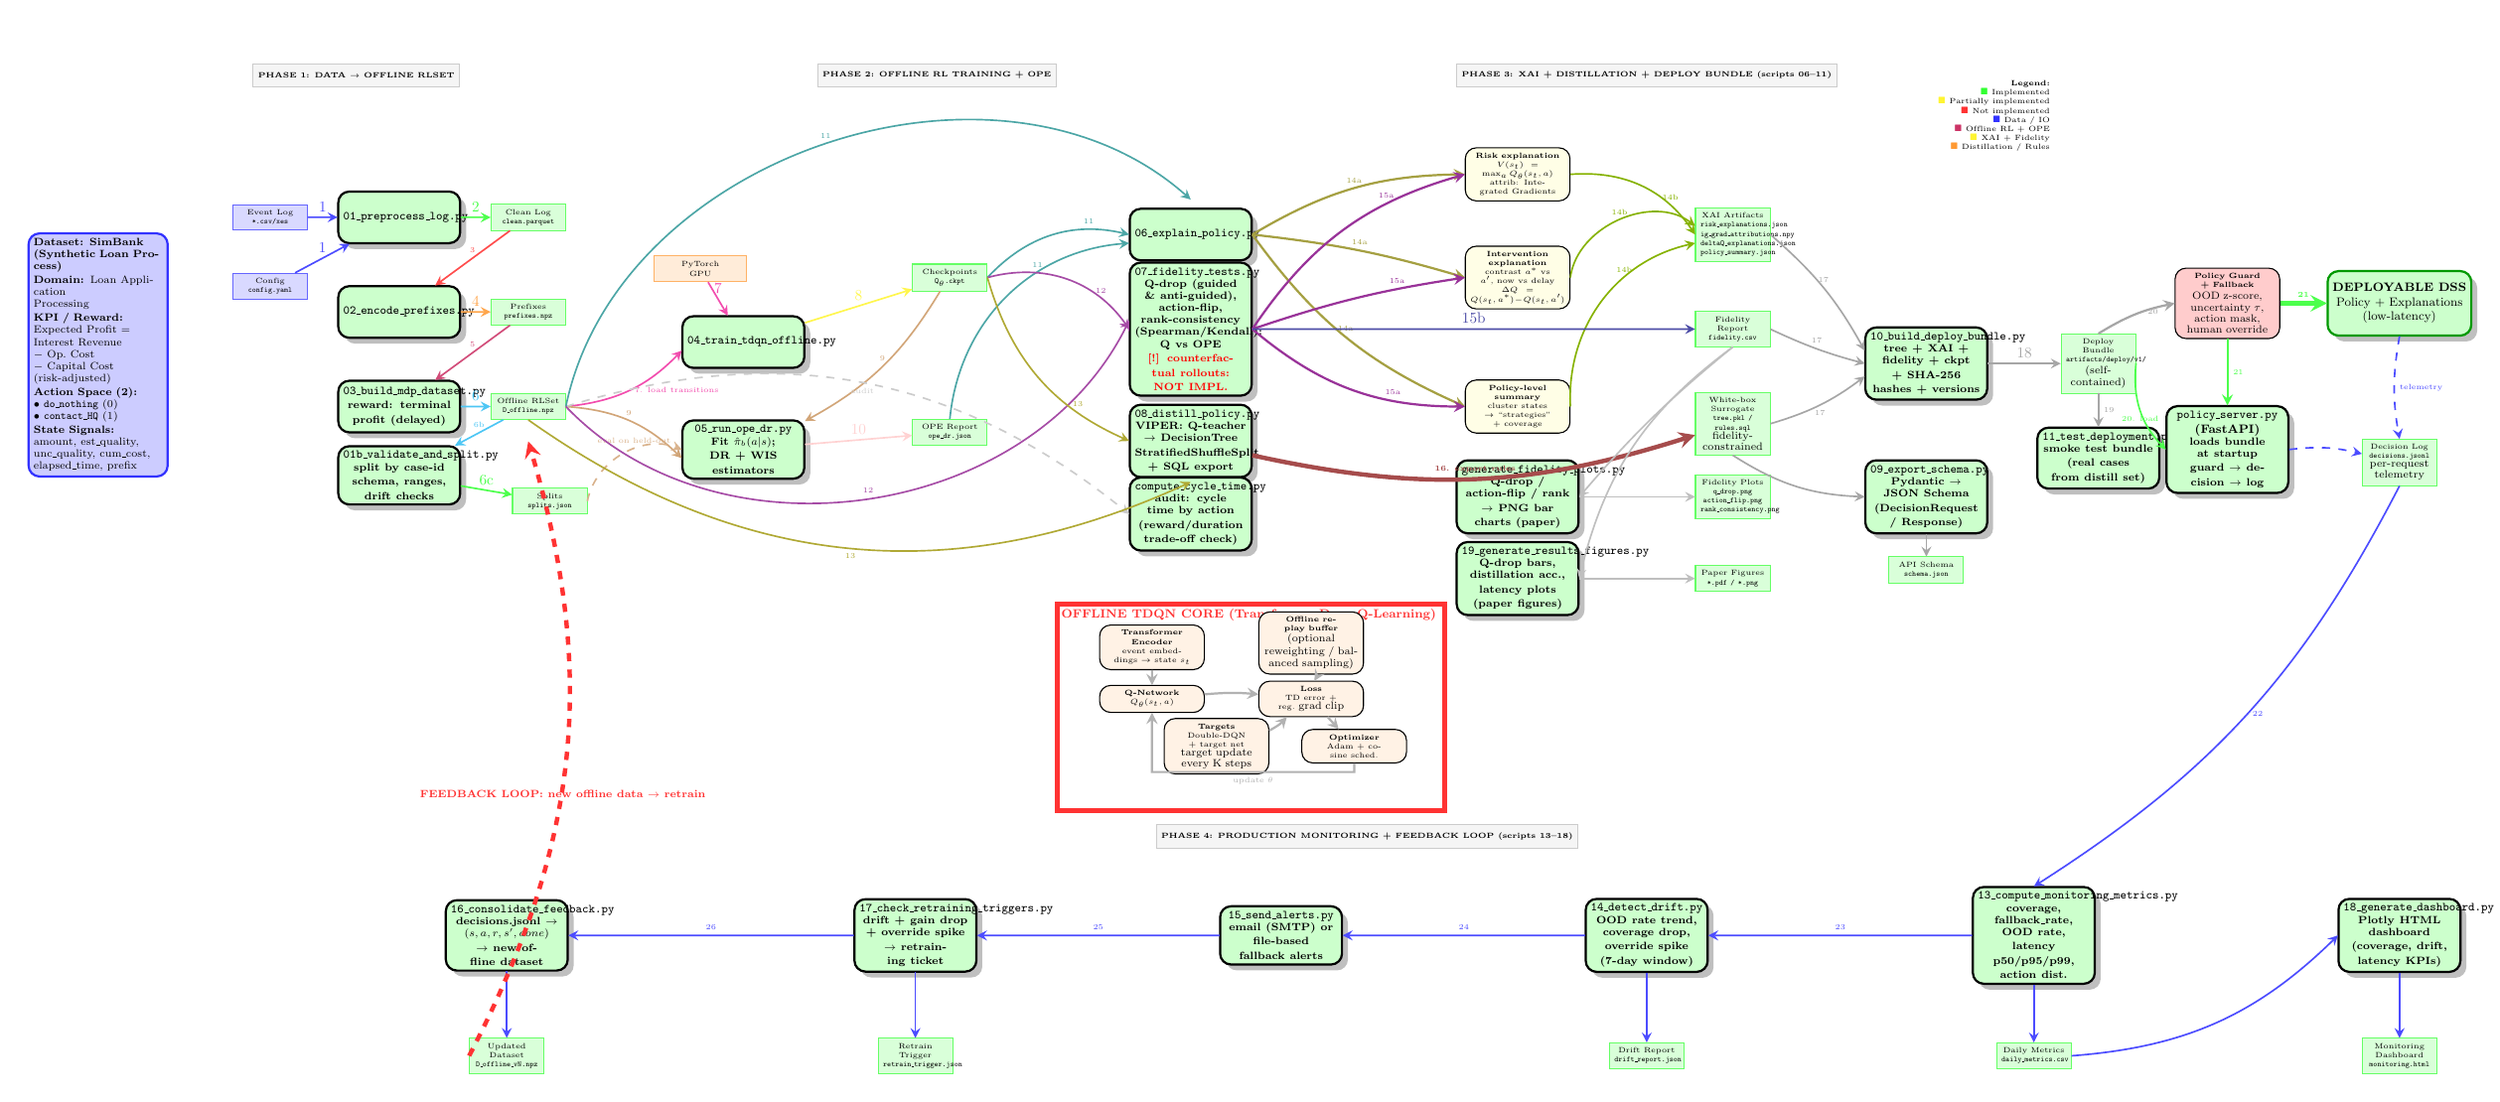
\begin{tikzpicture}[
    scale=0.55,
    transform shape,
    node distance=0.8cm and 1.5cm,
    script/.style={rectangle, rounded corners, draw=black, thick,
                   minimum width=2.8cm, minimum height=1.2cm,
                   text width=2.6cm, align=center, font=\footnotesize\bfseries, drop shadow},
    procstep/.style={rectangle, rounded corners, draw=black, fill=gray!10,
                   minimum width=2.4cm, minimum height=0.6cm,
                   text width=2.2cm, align=center, font=\tiny},
    input/.style={rectangle, draw=blue!60, fill=blue!15,
                   minimum width=1.7cm, minimum height=0.5cm,
                   text width=1.5cm, align=center, font=\tiny},
    output/.style={rectangle, draw=green!60, fill=green!15,
                    minimum width=1.7cm, minimum height=0.5cm,
                    text width=1.5cm, align=center, font=\tiny},
    tool/.style={rectangle, draw=orange!60, fill=orange!15,
                   minimum width=2.1cm, minimum height=0.6cm,
                   text width=1.9cm, align=center, font=\tiny},
    arrow/.style={->, >=stealth, semithick},
    phase/.style={rectangle, draw=gray!40, fill=gray!8,
                   minimum width=3.4cm, minimum height=0.55cm,
                   font=\tiny\bfseries, align=center},
    internal/.style={->, >=stealth, thin, gray!60},
    dataset/.style={rectangle, draw=blue!80, fill=blue!20, thick, rounded corners,
                   minimum width=3.2cm, minimum height=3.0cm,
                   text width=3.0cm, align=left, font=\scriptsize},
    implemented/.style={fill=green!20},
    partial/.style={fill=yellow!20},
    notimpl/.style={fill=red!20, dashed}
  ]

    % ===================== PHASE LABELS =====================
    \node[phase] (p1) at (-16, 10.5) {PHASE 1: DATA $\rightarrow$ OFFLINE RLSET};
    \node[phase] (p2) at (-2.5, 10.5) {PHASE 2: OFFLINE RL TRAINING + OPE};
    \node[phase] (p3) at (14.0, 10.5) {PHASE 3: XAI + DISTILLATION + DEPLOY BUNDLE (scripts 06--11)};
    \node[phase] (p4) at (7.5, -7.2)  {PHASE 4: PRODUCTION MONITORING + FEEDBACK LOOP (scripts 13--18)};

    % ===================== PHASE 1 =====================
    \node[dataset] (simbank) at (-22, 4) {
      \textbf{Dataset: SimBank}\\
      \textbf{(Synthetic Loan Process)}\\[1pt]
      \textbf{Domain:} Loan Application\\Processing\\[1pt]
      \textbf{KPI / Reward:}\\
      Expected Profit =\\
      Interest Revenue\\
      $-$ Op.\ Cost\\
      $-$ Capital Cost\\
      (risk-adjusted)\\[1pt]
      \textbf{Action Space (2):}\\
      $\bullet$ \texttt{do\_nothing} (0)\\
      $\bullet$ \texttt{contact\_HQ} (1)\\[1pt]
      \textbf{State Signals:}\\
      amount, est\_quality,\\
      unc\_quality, cum\_cost,\\
      elapsed\_time, prefix
    };

    \node[input] (logcsv) at (-18, 7.2) {Event Log\\\texttt{*.csv/xes}};
    \node[input] (cfg)    at (-18, 5.6) {Config\\\texttt{config.yaml}};

    \node[script, implemented] (prep)     at (-15, 7.2) {\texttt{01\_preprocess\_log.py}};
    \node[script, implemented] (encode)   at (-15, 5.0) {\texttt{02\_encode\_prefixes.py}};
    \node[script, implemented] (buildmdp) at (-15, 2.8) {\texttt{03\_build\_mdp\_dataset.py}\\
      \scriptsize reward: terminal profit (delayed)};

    \node[output] (cleanlog) at (-12, 7.2) {Clean Log\\\texttt{clean.parquet}};
    \node[output] (prefixes) at (-12, 5.0) {Prefixes\\\texttt{prefixes.npz}};
    \node[output] (rlset)    at (-12, 2.8) {Offline RLSet\\\texttt{D\_offline.npz}};

    \node[script, implemented] (validate) at (-15, 1.2) {\texttt{01b\_validate\_and\_split.py}\\
      \scriptsize split by case-id\\
      \scriptsize schema, ranges, drift checks};
    \node[output] (splits) at (-11.5, 0.6) {Splits\\\texttt{splits.json}};

    \draw[arrow, blue!70]   (logcsv)   -- node[midway, above] {1}  (prep);
    \draw[arrow, blue!70]   (cfg)      -- node[midway, above] {1}  (prep);
    \draw[arrow, green!70]  (prep)     -- node[midway, above] {2}  (cleanlog);
    \draw[arrow, red!70]    (cleanlog) -- node[midway, above, font=\tiny] {3} (encode);
    \draw[arrow, orange!70] (encode)   -- node[midway, above] {4}  (prefixes);
    \draw[arrow, purple!70] (prefixes) -- node[midway, above, font=\tiny] {5} (buildmdp);
    \draw[arrow, cyan!70]   (buildmdp) -- node[midway, above] {6}  (rlset);
    \draw[arrow, cyan!70]   (rlset)    -- node[midway, above, font=\tiny] {6b} (validate);
    \draw[arrow, green!70]  (validate) -- node[midway, above] {6c} (splits);

    % ===================== PHASE 2 =====================
    \node[script, implemented] (train) at (-7.0, 4.3) {\texttt{04\_train\_tdqn\_offline.py}};
    \node[tool] (gpu) at (-8.0, 6.0) {PyTorch\\GPU};
    \node[output] (ckpt) at (-2.2, 5.8) {Checkpoints\\\texttt{Q$_\theta$.ckpt}};

    \draw[arrow, magenta!70] (gpu)  -- node[midway, above] {7} (train);
    \draw[arrow, magenta!70] (rlset.east) to[bend left=-20]
      node[midway, right, font=\tiny] {7. load transitions} ([yshift=-2mm]train.west);
    \draw[arrow, yellow!70]  (train) -- node[midway, above] {8} (ckpt);

    % --- BIG BOX: OFFLINE RL CORE ---
    \node[rectangle, draw=red!80, ultra thick, fill=white,
          minimum width=9.0cm, minimum height=4.8cm] (core) at (4.8, -4.2) {};
    \node[anchor=north west, font=\footnotesize\bfseries, text=red!80] at (core.north west)
      {OFFLINE TDQN CORE (Transformer Deep Q-Learning)};

    \node[procstep, fill=orange!10] (encT)    at (2.5, -2.8)
      {\textbf{Transformer Encoder}\\event embeddings $\rightarrow$ state $s_t$};
    \node[procstep, fill=orange!10] (qnet)    at (2.5, -4.0)
      {\textbf{Q-Network}\\$Q_\theta(s_t,a)$};
    \node[procstep, fill=orange!10] (targets) at (4.0, -5.1)
      {\textbf{Targets}\\Double-DQN + target net\\
      \scriptsize target update every K steps};
    \node[procstep, fill=orange!10] (replay)  at (6.2, -2.7)
      {\textbf{Offline replay buffer}\\
      \scriptsize (optional reweighting / balanced sampling)};
    \node[procstep, fill=orange!10] (loss)    at (6.2, -4.0)
      {\textbf{Loss}\\TD error + reg.\ \scriptsize grad clip};
    \node[procstep, fill=orange!10] (opt)     at (7.2, -5.1)
      {\textbf{Optimizer}\\Adam + cosine sched.};

    \draw[internal, thick] (encT)   -- (qnet);
    \draw[internal, thick] (replay)  to[bend left=10]  (loss);
    \draw[internal, thick] (targets) to[bend right=10] (loss);
    \draw[internal, thick] (qnet)    to[bend left=5]   (loss);
    \draw[internal, thick] (loss)  -- (opt);
    \draw[internal, thick] (opt) -- ++(0,-0.6) -|
      node[pos=0.25, below, font=\tiny] {update $\theta$} (qnet.south);

    % --- OPE (Doubly Robust) ---
    \node[script, implemented] (ope) at (-7.0, 1.8)
      {\texttt{05\_run\_ope\_dr.py}\\
      \scriptsize Fit $\hat{\pi}_b(a|s)$;\\
      \scriptsize DR + WIS estimators};
    \node[output] (operep) at (-2.2, 2.2) {OPE Report\\\texttt{ope\_dr.json}};

    \draw[arrow, brown!70] (ckpt) to[bend left=15]
      node[midway, above, font=\tiny] {9} (ope);
    \draw[arrow, brown!70] (rlset.east) to[bend right=-20]
      node[midway, above, font=\tiny] {9} ([yshift=-2mm]ope.west);
    \draw[arrow, brown!60, dashed] (splits.east) to[bend left=50]
      node[pos=0.6, above, font=\tiny] {eval on held-out} (ope.west);
    \draw[arrow, pink!70] (ope) -- node[midway, above] {10} (operep);

    % ===================== PHASE 3 =====================
    \node[script, implemented] (xai) at (3.4, 6.8)
      {\texttt{06\_explain\_policy.py}};
    \node[script, implemented] (fidelity) at (3.4, 4.6)
      {\texttt{07\_fidelity\_tests.py}\\
      \scriptsize Q-drop (guided \& anti-guided),\\
      \scriptsize action-flip, rank-consistency\\
      \scriptsize (Spearman/Kendall): Q vs OPE\\
      \scriptsize \textcolor{red}{\textbf{[!]} counterfactual rollouts: NOT IMPL.}};
    \node[script, implemented] (distill) at (3.4, 2.0)
      {\texttt{08\_distill\_policy.py}\\
      \scriptsize VIPER: Q-teacher $\rightarrow$ DecisionTree\\
      \scriptsize StratifiedShuffleSplit + SQL export};

    \node[procstep, fill=yellow!10] (riskexp) at (11.0, 8.2)
      {\textbf{Risk explanation}\\
      $V(s_t)=\max_a Q_\theta(s_t,a)$\\
      attrib: Integrated Gradients};
    \node[procstep, fill=yellow!10] (intervexp) at (11.0, 5.8)
      {\textbf{Intervention explanation}\\
      contrast $a^*$ vs $a'$, now vs delay\\
      $\Delta Q = Q(s_t,a^*)-Q(s_t,a')$};
    \node[procstep, fill=yellow!10] (polsum) at (11.0, 2.8)
      {\textbf{Policy-level summary}\\
      cluster states $\rightarrow$ ``strategies''\\
      + coverage};

    \node[output] (xaiout) at (16.0, 6.8)
      {XAI Artifacts\\\texttt{risk\_explanations.json}\\
      \texttt{ig\_grad\_attributions.npy}\\\texttt{deltaQ\_explanations.json}\\\texttt{policy\_summary.json}};
    \node[output] (fidout)   at (16.0, 4.6)
      {Fidelity Report\\\texttt{fidelity.csv}};
    \node[output] (whitebox) at (16.0, 2.4)
      {White-box Surrogate\\\texttt{tree.pkl / rules.sql}\\
      \scriptsize fidelity-constrained};

    % Research/paper utility scripts
    \node[script, implemented] (fidplots) at (11.0, 0.7)
      {\texttt{generate\_fidelity\_plots.py}\\
      \scriptsize Q-drop / action-flip / rank\\
      \scriptsize $\rightarrow$ PNG bar charts (paper)};
    \node[output] (fidplotsout) at (16.0, 0.7)
      {Fidelity Plots\\\texttt{q\_drop.png}\\
      \texttt{action\_flip.png}\\
      \texttt{rank\_consistency.png}};

    \node[script, implemented] (figscript) at (11.0, -1.2)
      {\texttt{19\_generate\_results\_figures.py}\\
      \scriptsize Q-drop bars, distillation acc.,\\
      \scriptsize latency plots (paper figures)};
    \node[output] (figout) at (16.0, -1.2)
      {Paper Figures\\\texttt{*.pdf / *.png}};

    \node[script, implemented] (cycletime) at (3.4, 0.3)
      {\texttt{compute\_cycle\_time.py}\\
      \scriptsize audit: cycle time by action\\
      \scriptsize (reward/duration trade-off check)};

    % XAI internal connections
    \draw[internal, thick, yellow!60!black] (xai.east) to[bend left=15]
      node[pos=0.5, above, font=\tiny] {14a} (riskexp.west);
    \draw[internal, thick, yellow!60!black] (xai.east) to[bend left=5]
      node[pos=0.5, above, font=\tiny] {14a} (intervexp.west);
    \draw[internal, thick, yellow!60!black] (xai.east) to[bend right=15]
      node[pos=0.5, above, font=\tiny] {14a} (polsum.west);

    \draw[internal, thick, violet!80] (fidelity.east) to[bend left=20]
      node[pos=0.7, above, font=\tiny] {15a} (riskexp.west);
    \draw[internal, thick, violet!80] (fidelity.east) to[bend left=5]
      node[pos=0.7, above, font=\tiny] {15a} (intervexp.west);
    \draw[internal, thick, violet!80] (fidelity.east) to[bend right=20]
      node[pos=0.7, above, font=\tiny] {15a} (polsum.west);

    \draw[arrow, lime!70!black] (riskexp.east)  to[bend left=30]
      node[pos=0.75, above, font=\tiny] {14b} (xaiout.west);
    \draw[arrow, lime!70!black] (intervexp.east) to[bend left=60]
      node[midway, above, font=\tiny]   {14b} ([yshift=2mm]xaiout.west);
    \draw[arrow, lime!70!black] (polsum.east)   to[bend left=40]
      node[pos=0.65, above, font=\tiny] {14b} ([yshift=-2mm]xaiout.west);

    \draw[arrow, NavyBlue!70] (fidelity) -- node[midway, above] {15b} (fidout);
    \draw[arrow, Maroon!70, ultra thick] (distill)
      to[bend right=15] node[midway, above, font=\tiny\bfseries] {16. export rules} (whitebox);

    % Research utilities
    \draw[arrow, gray!50] (fidout.south) to[bend right=5]
      (fidplots.east);
    \draw[arrow, gray!50] (fidplots.east) -- (fidplotsout.west);
    \draw[arrow, gray!50] (fidout.south) to[bend right=20]
      (figscript.east);
    \draw[arrow, gray!50] (figscript.east) -- (figout.west);
    \draw[arrow, gray!40, dashed] (rlset.east) to[bend right=-28]
      node[midway, below, font=\tiny] {audit} (cycletime.west);

    % Inputs to XAI / distill from Phase 2
    \draw[arrow, teal!70] (ckpt.east) to[bend left=30]
      node[pos=0.75, above, font=\tiny] {11} (xai.west);
    \draw[arrow, teal!70] (rlset.east) to[bend left=60]
      node[midway, above, font=\tiny] {11} ([yshift=2mm]xai.north);
    \draw[arrow, teal!70] (operep.north) to[bend left=40]
      node[pos=0.65, above, font=\tiny] {11} ([yshift=-2mm]xai.west);

    \draw[arrow, violet!70] (ckpt.east) to[bend left=35]
      node[pos=0.75, above, font=\tiny] {12} (fidelity.west);
    \draw[arrow, violet!70] (rlset.east) to[bend left=-55]
      node[midway, above, font=\tiny] {12} ([yshift=2mm]fidelity.west);

    \draw[arrow, olive!70] (ckpt.east) to[bend right=25]
      node[pos=0.75, above, font=\tiny] {13} (distill.west);
    \draw[arrow, olive!70] (rlset.south) to[bend left=-30]
      node[midway, below, font=\tiny] {13} ([yshift=-1mm]distill.south);

    % ===================== DEPLOY CHAIN: scripts 09, 10, 11 =====================
    % 09 — export schema
    \node[script, implemented] (exportschema) at (20.5, 0.7)
      {\texttt{09\_export\_schema.py}\\
      \scriptsize Pydantic $\rightarrow$ JSON Schema\\
      \scriptsize (DecisionRequest / Response)};
    \node[output] (schema) at (20.5, -1.0)
      {API Schema\\\texttt{schema.json}};

    % 10 — build deploy bundle
    \node[script, implemented] (buildbundle) at (20.5, 3.8)
      {\texttt{10\_build\_deploy\_bundle.py}\\
      \scriptsize tree + XAI + fidelity + ckpt\\
      \scriptsize + SHA-256 hashes + versions};
    \node[output] (bundle) at (24.5, 3.8)
      {Deploy Bundle\\\texttt{artifacts/deploy/v1/}\\
      \scriptsize (self-contained)};

    % 11 — test deployment
    \node[script, implemented] (testdeploy) at (24.5, 1.6)
      {\texttt{11\_test\_deployment.py}\\
      \scriptsize smoke test bundle\\
      \scriptsize (real cases from distill set)};

    % Connections into 10_build_deploy_bundle
    \draw[arrow, gray!70] (xaiout.east)   to[bend left=10]
      node[pos=0.5, above, font=\tiny] {17} ([yshift=3mm]buildbundle.west);
    \draw[arrow, gray!70] (fidout.east)   to[bend left=-5]
      node[pos=0.5, above, font=\tiny] {17} (buildbundle.west);
    \draw[arrow, gray!70] (whitebox.east) to[bend right=10]
      node[pos=0.5, below, font=\tiny] {17} ([yshift=-3mm]buildbundle.west);
    \draw[arrow, gray!70] (buildbundle.east) -- node[midway, above] {18} (bundle.west);
    \draw[arrow, gray!70] (bundle.south)     -- node[midway, right, font=\tiny] {19} (testdeploy.north);

    % 09 schema connections
    \draw[arrow, gray!70] (whitebox.south) to[bend right=15]
      node[pos=0.5, right, font=\tiny] {} (exportschema.west);
    \draw[arrow, gray!70] (exportschema.south) -- (schema.north);

    % ===================== POLICY GUARD + SERVER =====================
    \node[procstep, fill=red!20] (guard) at (27.5, 5.2)
      {\textbf{Policy Guard + Fallback}\\
      \scriptsize OOD z-score, uncertainty $\tau$,\\
      \scriptsize action mask, human override};

    \node[script, implemented] (policyapi) at (27.5, 1.8)
      {\texttt{policy\_server.py} (FastAPI)\\
      \scriptsize loads bundle at startup\\
      \scriptsize guard $\rightarrow$ decision $\rightarrow$ log};

    \node[rectangle, draw=green!60!black, fill=green!20, thick, rounded corners,
          minimum width=3.0cm, minimum height=1.5cm, drop shadow, align=center,
          font=\footnotesize] (deploy) at (31.5, 5.2)
      {\textbf{DEPLOYABLE DSS}\\Policy + Explanations\\(low-latency)};

    % Bundle → guard, server, deploy
    \draw[arrow, gray!70, thick] (bundle.north) to[bend left=10]
      node[pos=0.6, right, font=\tiny] {20} (guard.west);
    \draw[arrow, green!70] (bundle.east) to[bend right=25]
      node[pos=0.5, below, font=\tiny] {20. load} (policyapi.west);
    \draw[arrow, green!70, thick] (guard.south) --
      node[midway, right, font=\tiny] {21} (policyapi.north);
    \draw[arrow, green!70, ultra thick] (guard.east) --
      node[midway, above, font=\tiny\bfseries] {21} (deploy.west);

    % ===================== PHASE 4: MONITORING =====================
    \node[output] (declog) at (31.5, 1.5)
      {Decision Log\\\texttt{decisions.jsonl}\\
      \scriptsize per-request telemetry};
    \draw[arrow, blue!70, dashed] (deploy.south)   to[bend right=10]
      node[midway, right, font=\tiny] {telemetry} (declog.north);
    \draw[arrow, blue!70, dashed] (policyapi.east) to[bend left=10]
      ([yshift=2mm]declog.west);

    % Script 13
    \node[script, implemented] (monmetrics) at (23.0, -9.5)
      {\texttt{13\_compute\_monitoring\_metrics.py}\\
      \scriptsize coverage, fallback\_rate, OOD rate,\\
      \scriptsize latency p50/p95/p99, action dist.};
    \node[output] (metricsout) at (23.0, -12.3)
      {Daily Metrics\\\texttt{daily\_metrics.csv}};

    % Script 14
    \node[script, implemented] (detectdrift) at (14.0, -9.5)
      {\texttt{14\_detect\_drift.py}\\
      \scriptsize OOD rate trend, coverage drop,\\
      \scriptsize override spike (7-day window)};
    \node[output] (driftout) at (14.0, -12.3)
      {Drift Report\\\texttt{drift\_report.json}};

    % Script 15
    \node[script, implemented] (sendalerts) at (5.5, -9.5)
      {\texttt{15\_send\_alerts.py}\\
      \scriptsize email (SMTP) or\\
      \scriptsize file-based fallback alerts};

    % Script 17
    \node[script, implemented] (retriggers) at (-3.0, -9.5)
      {\texttt{17\_check\_retraining\_triggers.py}\\
      \scriptsize drift + gain drop + override spike\\
      \scriptsize $\rightarrow$ retraining ticket};
    \node[output] (trigout) at (-3.0, -12.3)
      {Retrain Trigger\\\texttt{retrain\_trigger.json}};

    % Script 16 (feedback → offline dataset)
    \node[script, implemented] (consolid) at (-12.5, -9.5)
      {\texttt{16\_consolidate\_feedback.py}\\
      \scriptsize decisions.jsonl $\rightarrow$ $(s,a,r,s',done)$\\
      \scriptsize $\rightarrow$ new offline dataset};
    \node[output] (fbout) at (-12.5, -12.3)
      {Updated Dataset\\\texttt{D\_offline\_vN.npz}};

    % Script 18 (dashboard)
    \node[script, implemented] (gendash) at (31.5, -9.5)
      {\texttt{18\_generate\_dashboard.py}\\
      \scriptsize Plotly HTML dashboard\\
      \scriptsize (coverage, drift, latency KPIs)};
    \node[output] (dashout) at (31.5, -12.3)
      {Monitoring Dashboard\\\texttt{monitoring.html}};

    % Phase 4 flow (right-to-left = feedback direction)
    \draw[arrow, blue!70] (declog.south) to[bend left=15]
      node[midway, right, font=\tiny] {22} (monmetrics.north);
    \draw[arrow, blue!70] (monmetrics.south) -- node[midway, right, font=\tiny] {} (metricsout.north);
    \draw[arrow, blue!70] (monmetrics)       -- node[midway, above, font=\tiny] {23} (detectdrift);
    \draw[arrow, blue!70] (detectdrift.south)-- node[midway, right, font=\tiny] {} (driftout.north);
    \draw[arrow, blue!70] (detectdrift)      -- node[midway, above, font=\tiny] {24} (sendalerts);
    \draw[arrow, blue!70] (sendalerts)       -- node[midway, above, font=\tiny] {25} (retriggers);
    \draw[arrow, blue!70] (retriggers.south) -- node[midway, right, font=\tiny] {} (trigout.north);
    \draw[arrow, blue!70] (retriggers)       -- node[midway, above, font=\tiny] {26} (consolid);
    \draw[arrow, blue!70] (consolid.south)   -- node[midway, right, font=\tiny] {} (fbout.north);
    \draw[arrow, blue!70] (metricsout.east) to[bend right=20]
      node[pos=0.5, below, font=\tiny] {} (gendash.west);
    \draw[arrow, blue!70] (gendash.south)   -- (dashout.north);

    % Feedback loop → Phase 1 / 2
    \draw[arrow, red!80, ultra thick, dashed] (fbout.west)
      to[bend right=22]
      node[pos=0.45, below, font=\scriptsize\bfseries]
        {FEEDBACK LOOP: new offline data $\rightarrow$ retrain}
      ([yshift=-5mm]rlset.south);

    % Legend
    \node[anchor=north east, font=\tiny, align=right] at (23.5, 10.5) {
        \textbf{Legend:}\\
        \textcolor{green!80}{$\blacksquare$} Implemented\\
        \textcolor{yellow!80}{$\blacksquare$} Partially implemented\\
        \textcolor{red!80}{$\blacksquare$} Not implemented\\
        \textcolor{blue!80}{$\blacksquare$} Data / IO\\
        \textcolor{purple!80}{$\blacksquare$} Offline RL + OPE\\
        \textcolor{yellow!80}{$\blacksquare$} XAI + Fidelity\\
        \textcolor{orange!80}{$\blacksquare$} Distillation / Rules
    };

  \end{tikzpicture}
  }

  \caption{
\textbf{End-to-end implementation architecture (actual state) of xPPM-TDQN:
Explainable Prescriptive Process Monitoring with Transformer Deep Q-Learning.}
All coloured boxes are fully implemented.
\textbf{Phase 1} preprocesses SimBank event logs (2-action space:
\texttt{do\_nothing} vs \texttt{contact\_HQ}),
encodes prefixes, builds the MDP dataset with terminal-profit reward,
and produces stratified train/val/test splits.
\textbf{Phase 2} trains an offline Double-DQN with a Transformer encoder
(d\_model=128, 4 heads, 3 layers) and evaluates the learned policy
off-policy with doubly robust + WIS estimators.
\textbf{Phase 3} generates three explanation types
(risk via Integrated Gradients, $\Delta Q$ contrastive, policy-level clustering),
runs fidelity tests (Q-drop guided \& anti-guided, action-flip, rank-consistency
Spearman/Kendall),
distills the Q-teacher to a decision tree via VIPER
(StratifiedShuffleSplit + SQL rule export),
exports the API JSON Schema (script 09),
bundles all artifacts with SHA-256 content hashes (script 10),
and smoke-tests the bundle on real distillation cases (script 11).
The FastAPI server loads the bundle at startup and filters every decision
through a Policy Guard (OOD z-score, uncertainty threshold, action mask, human override).
\textbf{Phase 4} closes the production loop: the server logs each decision to
\texttt{decisions.jsonl}; scripts 13--18 compute daily metrics,
detect drift (OOD trend, coverage drop, override spike), dispatch alerts,
check retraining triggers, consolidate feedback into a new offline dataset
(\texttt{D\_offline\_vN.npz}), and generate a Plotly monitoring dashboard.
Research utilities (\texttt{generate\_fidelity\_plots.py},
\texttt{19\_generate\_results\_figures.py},
\texttt{compute\_cycle\_time.py}) are shown separately.
\textbf{Note:} Counterfactual rollouts in fidelity tests are not yet implemented.
  }
  \label{fig:code_architecture_actual}
\end{figure}

\end{document}
